% Options for packages loaded elsewhere
\PassOptionsToPackage{unicode}{hyperref}
\PassOptionsToPackage{hyphens}{url}
%
\documentclass[
]{article}
\usepackage{amsmath,amssymb}
\usepackage{iftex}
\ifPDFTeX
  \usepackage[T5]{fontenc}
  \usepackage[utf8]{inputenc}
  \usepackage{textcomp} % provide euro and other symbols
\else % if luatex or xetex
  \usepackage{unicode-math} % this also loads fontspec
  \defaultfontfeatures{Scale=MatchLowercase}
  \defaultfontfeatures[\rmfamily]{Ligatures=TeX,Scale=1}
\fi
\usepackage{lmodern}
\ifPDFTeX\else
  % xetex/luatex font selection
\fi
% Use upquote if available, for straight quotes in verbatim environments
\IfFileExists{upquote.sty}{\usepackage{upquote}}{}
\IfFileExists{microtype.sty}{% use microtype if available
  \usepackage[]{microtype}
  \UseMicrotypeSet[protrusion]{basicmath} % disable protrusion for tt fonts
}{}
\makeatletter
\@ifundefined{KOMAClassName}{% if non-KOMA class
  \IfFileExists{parskip.sty}{%
    \usepackage{parskip}
  }{% else
    \setlength{\parindent}{0pt}
    \setlength{\parskip}{6pt plus 2pt minus 1pt}}
}{% if KOMA class
  \KOMAoptions{parskip=half}}
\makeatother
\usepackage{xcolor}
\usepackage{longtable,booktabs,array}
\usepackage{calc} % for calculating minipage widths
% Correct order of tables after \paragraph or \subparagraph
\usepackage{etoolbox}
\makeatletter
\patchcmd\longtable{\par}{\if@noskipsec\mbox{}\fi\par}{}{}
\makeatother
% Allow footnotes in longtable head/foot
\IfFileExists{footnotehyper.sty}{\usepackage{footnotehyper}}{\usepackage{footnote}}
\makesavenoteenv{longtable}
\usepackage{graphicx}
\makeatletter
\newsavebox\pandoc@box
\newcommand*\pandocbounded[1]{% scales image to fit in text height/width
  \sbox\pandoc@box{#1}%
  \Gscale@div\@tempa{\textheight}{\dimexpr\ht\pandoc@box+\dp\pandoc@box\relax}%
  \Gscale@div\@tempb{\linewidth}{\wd\pandoc@box}%
  \ifdim\@tempb\p@<\@tempa\p@\let\@tempa\@tempb\fi% select the smaller of both
  \ifdim\@tempa\p@<\p@\scalebox{\@tempa}{\usebox\pandoc@box}%
  \else\usebox{\pandoc@box}%
  \fi%
}
% Set default figure placement to H (non-floating)
\usepackage{float}
\def\fps@figure{H}
\makeatother
\setlength{\emergencystretch}{3em} % prevent overfull lines
\providecommand{\tightlist}{%
  \setlength{\itemsep}{0pt}\setlength{\parskip}{0pt}}
\setcounter{secnumdepth}{-\maxdimen} % remove section numbering
\usepackage{bookmark}
\IfFileExists{xurl.sty}{\usepackage{xurl}}{} % add URL line breaks if available
\urlstyle{same}
\hypersetup{
  hidelinks,
  pdfcreator={LaTeX via pandoc}}

\author{}
\date{}

\begin{document}

\section{Round 2 Executive Summary \& Narrative
Analysis}\label{round-2-executive-summary-narrative-analysis}

\subsection{Executive Summary}\label{executive-summary}

This report provides the outbound flow analysis, customer profiling, and
geographic demand mapping for the Round 2 competition based on the
transaction logs spanning June to December 2025. The core analysis
focuses on the 6-month Assignment Window (July 1 -- December 31, 2025),
which contains \textbf{43,894 shipment rows}, \textbf{355,364.80 units
of outbound demand}, and \textbf{19,653.78 CBM of volume}.

Key takeaways include: 1. \textbf{Extreme Assortment Concentration}: A
tiny fraction of SKUs drives the vast majority of volume and warehouse
activities. A dedicated `Fast-Moving' group of 59 SKUs accounts for
65.06\% of outbound quantity and 49.61\% of order frequency. 2.
\textbf{ERP Centralized Invoicing Distortion}: Geographic demand
analyses reveal that My Phuoc seemingly dominates 92.22\% of resolved
volume. However, this is an artificial bias caused by centralized ERP
invoicing. In reality, Vinh Loc's raw outbound shipments account for
28.75\% of total volume, but 80.10\% of its transactions have missing
customer names and are excluded from standard maps. Using
\textbf{Approach A (Statistical Scaling)}, we restore and analyze the
true 71.25\% My Phuoc vs 28.75\% Vinh Loc volume split. 3. \textbf{Clear
Segment Profiles}: Modern Trade orders are large, consolidated, and
heavily palletized (69.17\% of quantity). Traditional Trade orders are
smaller, highly fragmented (51.49\% carton / 8.07\% loose), and spread
across 57 provinces, presenting different operational picking
requirements.

\begin{center}\rule{0.5\linewidth}{0.5pt}\end{center}

\subsection{Q1.1 Demand Pattern Classification (ABC-XYZ
Analysis)}\label{q1.1-demand-pattern-classification-abc-xyz-analysis}

The product assortment was analyzed across two dimensions using a joint
ABC-XYZ matrix based on outbound volume (Quantity) and transaction
frequency (Order Frequency) over the last 6 months of 2025. The overall
concentration of shipped volume across SKUs is shown in Figure
\ref{fig:q11-abc-qty-dist}.

\begin{figure}
\centering
\pandocbounded{
\includegraphics[keepaspectratio]{../charts/q11_abc_quantity_distribution.png}}
\caption{Q1.1 ABC quantity distribution\label{fig:q11-abc-qty-dist}}
\end{figure}

\subsubsection{Classification
Thresholds}\label{classification-thresholds}

\begin{itemize}
\tightlist
\item
  \textbf{ABC Quantity Thresholds}: Class A (Top 80\%), Class B (Next
  15\%), Class C (Bottom 5\%)
\item
  \textbf{XYZ Variability Thresholds}: Class X (CV \(\le\) 0.50), Class
  Y (CV \(\le\) 1.00), Class Z (CV \textgreater{} 1.00 or Low Sample)
\item
  \textbf{Low-Sample Filter}: SKUs with fewer than 4 nonzero sales weeks
  are automatically downgraded to Class Z to prevent statistical skew.
\end{itemize}

\subsubsection{Joint ABC-XYZ Matrix
Summary}\label{joint-abc-xyz-matrix-summary}

A total of \textbf{572 unique SKUs} were classified. The product
distribution across the ABC-XYZ matrix is shown in the summary table
below:

\begin{longtable}[]{@{}
  >{\raggedright\arraybackslash}p{(\linewidth - 6\tabcolsep) * \real{0.2105}}
  >{\centering\arraybackslash}p{(\linewidth - 6\tabcolsep) * \real{0.2632}}
  >{\centering\arraybackslash}p{(\linewidth - 6\tabcolsep) * \real{0.2632}}
  >{\centering\arraybackslash}p{(\linewidth - 6\tabcolsep) * \real{0.2632}}@{}}
\toprule\noalign{}
\begin{minipage}[b]{\linewidth}\raggedright
XYZ ~ABC
\end{minipage} & \begin{minipage}[b]{\linewidth}\centering
Class A (Top 80\% Vol, 79 SKUs)
\end{minipage} & \begin{minipage}[b]{\linewidth}\centering
Class B (Next 15\% Vol, 118 SKUs)
\end{minipage} & \begin{minipage}[b]{\linewidth}\centering
Class C (Bottom 5\% Vol, 375 SKUs)
\end{minipage} \\
\midrule\noalign{}
\endhead
\bottomrule\noalign{}
\endlastfoot
\textbf{Class X} (Stable demand) & 1 SKUs (0.17\%) & 0 SKUs (0.00\%) & 0
SKUs (0.00\%) \\
\textbf{Class Y} (Variable demand) & 19 SKUs (3.32\%) & 19 SKUs (3.32\%)
& 9 SKUs (1.57\%) \\
\textbf{Class Z} (Irregular/Spiky) & 59 SKUs (10.31\%) & 99 SKUs
(17.31\%) & 366 SKUs (63.99\%) \\
\end{longtable}

\subsubsection{Identification of the `Fast-Moving' SKU
Group}\label{identification-of-the-fast-moving-sku-group}

The \textbf{Fast-Moving} SKU group is defined as the intersection of
Class A by Quantity and Class A by Order Frequency (Class A-A). This
group is the primary driver of warehouse operational workload and
inventory velocity.

\begin{itemize}
\tightlist
\item
  \textbf{SKU Count}: \textbf{59 SKUs} (representing \textbf{10.31\%} of
  the total assortment).
\item
  \textbf{Volume Contribution}: Accounts for \textbf{231211.92 units}
  (\textbf{65.06\%} of total outbound volume).
\item
  \textbf{Fulfillment Workload}: Drives \textbf{20615 orders}
  (\textbf{49.61\%} of all outbound transaction lines).
\item
  \textbf{Top 10 Fast-Moving SKUs}:
  \texttt{4200009163,\ 4200000163,\ 4200009000,\ 4200008101,\ 4200008999,\ 4200008102,\ 4200007858,\ 1830009179,\ 4200008229,\ 4200000164}.
\end{itemize}

\begin{quote}
{[}!TIP{]} \textbf{Operational Recommendation}: Because only
\textasciitilde10\% of the SKUs drive nearly 2/3 of all shipped
quantities, these 59 SKUs should be assigned to the most ergonomic
pick-faces (lower levels, close to the packing stations) with dedicated
replenishment pathways to minimize picking travel time.
\end{quote}

\begin{center}\rule{0.5\linewidth}{0.5pt}\end{center}

\subsection{Q1.2 Distribution Heatmap and Warehouse Imbalance
Analysis}\label{q1.2-distribution-heatmap-and-warehouse-imbalance-analysis}

\subsubsection{1. Data Quality and Resolution
Ceiling}\label{data-quality-and-resolution-ceiling}

A critical finding from our data cleansing pipeline is a \textbf{severe
geography resolution ceiling}: - \textbf{Row-level coverage}: Only
\textbf{36.69\%} of transaction rows (16,104 out of 43,894) could be
mapped to a known customer location. - \textbf{Quantity-level coverage}:
Only \textbf{44.92\%} of outbound quantities (159,635.70 out of
355,364.80) are linked to known coordinates. - \textbf{Root Cause}:
\texttt{27,790} assignment-window rows are unresolved, of which
\textbf{25,693 rows} are due to \texttt{Ship-to\ Customer} being logged
as \texttt{\textquotesingle{}unknown\textquotesingle{}} in the database.

\begin{quote}
{[}!IMPORTANT{]} \textbf{Central Invoicing Data Bias}: This missing
customer data is systemic: - \textbf{Centralization (Pre-Dec 2025)}:
Customer billing was centralized under My Phuoc's ERP account.
Consequently, Vinh Loc shipments (representing Tefal products) were
logged as internal stock depletion entries without customer details,
affecting \textbf{80.10\%} of Vinh Loc rows. - \textbf{Migration (Dec
2025)}: Billing migrated to Vinh Loc, causing My Phuoc's December
transactions to lack customer details. - \textbf{Operational Impact}:
Vinh Loc is left with an extremely low geographic coverage of
\textbf{12.12\% of its volume}, skewing all raw geographic charts to
make Vinh Loc look artificially inactive. This systematic bias and the
resulting spatial coverage limits are visualized in Figure
\ref{fig:q12-geo-coverage}.
\end{quote}

\begin{figure}
\centering
\pandocbounded{
\includegraphics[keepaspectratio]{../charts/q12_geography_coverage_map.png}}
\caption{Q1.2 Geography coverage map\label{fig:q12-geo-coverage}}
\end{figure}

\subsubsection{2. Corrected Warehouse Imbalance (Approach A: Statistical
Scaling)}\label{corrected-warehouse-imbalance-approach-a-statistical-scaling}

To provide a safe and unbiased view of warehouse throughput, we compare
raw volume totals against resolved volumes and apply \textbf{Approach A
(Statistical Scaling)}:

\begin{longtable}[]{@{}
  >{\raggedright\arraybackslash}p{(\linewidth - 6\tabcolsep) * \real{0.4356}}
  >{\centering\arraybackslash}p{(\linewidth - 6\tabcolsep) * \real{0.1881}}
  >{\centering\arraybackslash}p{(\linewidth - 6\tabcolsep) * \real{0.1881}}
  >{\centering\arraybackslash}p{(\linewidth - 6\tabcolsep) * \real{0.1881}}@{}}
\toprule\noalign{}
\begin{minipage}[b]{\linewidth}\raggedright
Metric
\end{minipage} & \begin{minipage}[b]{\linewidth}\centering
My Phuoc Warehouse
\end{minipage} & \begin{minipage}[b]{\linewidth}\centering
Vinh Loc Warehouse
\end{minipage} & \begin{minipage}[b]{\linewidth}\centering
Total
\end{minipage} \\
\midrule\noalign{}
\endhead
\bottomrule\noalign{}
\endlastfoot
\textbf{Raw Outbound Quantity} & 253,197.00 (71.25\%) & 102,167.80
(28.75\%) & 355,364.80 (100.0\%) \\
\textbf{Raw Outbound CBM} & 13,948.74 (70.97\%) & 5,705.04 (29.03\%) &
19,653.78 (100.0\%) \\
\textbf{Raw Transaction Rows} & 17,423 (39.70\%) & 26,471 (60.30\%) &
43,894 (100.0\%) \\
\textbf{Resolved Quantity (Raw)} & 147,258.80 (92.25\%) & 12,382.80
(7.75\%) & 159,635.70 (100.0\%) \\
\textbf{Imputed Quantity (Approach A)} & \textbf{253,196.01 (71.25\%)} &
\textbf{102,168.32 (28.75\%)} & \textbf{355,364.33 (100.0\%)} \\
\end{longtable}

\textbf{Conclusion}: While Vinh Loc represents 60.30\% of transaction
rows (small, frequent orders of Tefal items), it accounts for 28.75\% of
outbound quantity. My Phuoc handles 71.25\% of the quantity. The raw
resolved geography is heavily biased (92\% vs 8\%), but the true
operational split is \textbf{71\% My Phuoc vs 29\% Vinh Loc}. The
comparison of raw, resolved, and imputed throughput is detailed in the
table above, while the regional warehouse dominance gap in the resolved
transactions is shown in Figure \ref{fig:q12-wh-imbalance}.

\begin{figure}
\centering
\pandocbounded{
\includegraphics[keepaspectratio]{../charts/q12_warehouse_imbalance.png}}
\caption{Q1.2 Warehouse imbalance\label{fig:q12-wh-imbalance}}
\end{figure}

\subsubsection{3. Regional Demand and Top
Clusters}\label{regional-demand-and-top-clusters}

To define the geographic boundaries of our analysis, the standard
Vietnam administrative regions are mapped in Figure
\ref{fig:q12-vn-regions}.

\begin{figure}
\centering

\includegraphics[width=0.5\linewidth,height=\textheight,keepaspectratio]{../charts/q12_region_reference_map.png}
\caption{Q1.2 Vietnam regioning map\label{fig:q12-vn-regions}}
\end{figure}

Within these boundaries, the resolved outbound demand is highly
concentrated. As shown in Figure \ref{fig:q12-region-qty}, the
region-level order and quantity shares are led by the following regions:
- \textbf{Đông Nam Bộ}: The largest demand region, accounting for
\textbf{42.78\%} of resolved volume (68,289.44 units). - \textbf{Bắc
Trung Bộ và Duyên hải miền Trung}: The second largest, representing
\textbf{28.22\%} (45,044.48 units). - \textbf{Đồng bằng sông Cửu Long}:
Accounts for \textbf{13.86\%} (22,132.83 units).

\begin{figure}
\centering
\pandocbounded{
\includegraphics[keepaspectratio]{../charts/q12_region_quantity_orders.png}}
\caption{Q1.2 Regional quantity\label{fig:q12-region-qty}}
\end{figure}

\paragraph{Top Customer Clusters
(Provinces)}\label{top-customer-clusters-provinces}

At the provincial level, demand clusters heavily around key urban
centers. The absolute volume hotspots are highlighted in the top demand
provinces map (see Figure \ref{fig:q12-top-provinces}).

\begin{figure}
\centering

\includegraphics[width=0.5\linewidth,height=\textheight,keepaspectratio]{../charts/q12_top_demand_provinces_map.png}
\caption{Q1.2 Top demand provinces map\label{fig:q12-top-provinces}}
\end{figure}

Specifically, the top five provinces by resolved volume and order counts
are led by Hồ Chí Minh City by an overwhelming margin: - \textbf{Hồ Chí
Minh}: 1,267 orders, 42,256.09 quantity (representing \textbf{34.62\% of
resolved orders} and \textbf{26.47\% of resolved quantity}). -
\textbf{Đồng Nai}: 387 orders, 5,579.33 quantity. - \textbf{Bình Dương}:
194 orders, 19,814.17 quantity (high volume per order). - \textbf{Đà
Nẵng}: 204 orders, 15,522.98 quantity (Central hub). - \textbf{Cần Thơ}:
177 orders, 10,561.08 quantity (Mekong Delta hub).

To visualize the full provincial distribution across the nation, Figure
\ref{fig:q12-province-demand} displays the provincial demand choropleth
maps (by total quantity and total orders).

\begin{figure}
\centering
\pandocbounded{
\includegraphics[keepaspectratio]{../charts/q12_province_demand_choropleths.png}}
\caption{Q1.2 Province demand maps\label{fig:q12-province-demand}}
\end{figure}

\subsubsection{4. Fulfillment Splits and Spatial
Dynamics}\label{fulfillment-splits-and-spatial-dynamics}

To understand how fulfillment is shared between the facilities, we
examine the warehouse-region throughput split.

\paragraph{Warehouse-Region Fulfillment
Splits}\label{warehouse-region-fulfillment-splits}

Because My Phuoc holds Fans and Vinh Loc holds Tefal, both warehouses
ship to the same regions to fulfill their respective product lines. This
regional throughput distribution is visualized in Figure
\ref{fig:q12-wh-region-split}.

\begin{figure}
\centering
\pandocbounded{
\includegraphics[keepaspectratio]{../charts/q12_warehouse_region_quantity_split.png}}
\caption{Q1.2 Warehouse-region split\label{fig:q12-wh-region-split}}
\end{figure}

However, due to the centralized billing bias, My Phuoc appears dominant
in almost all regions. This dominance pattern and the resulting spatial
market coverage of both warehouses are mapped in Figure
\ref{fig:q12-wh-dominance}.

\begin{figure}
\centering
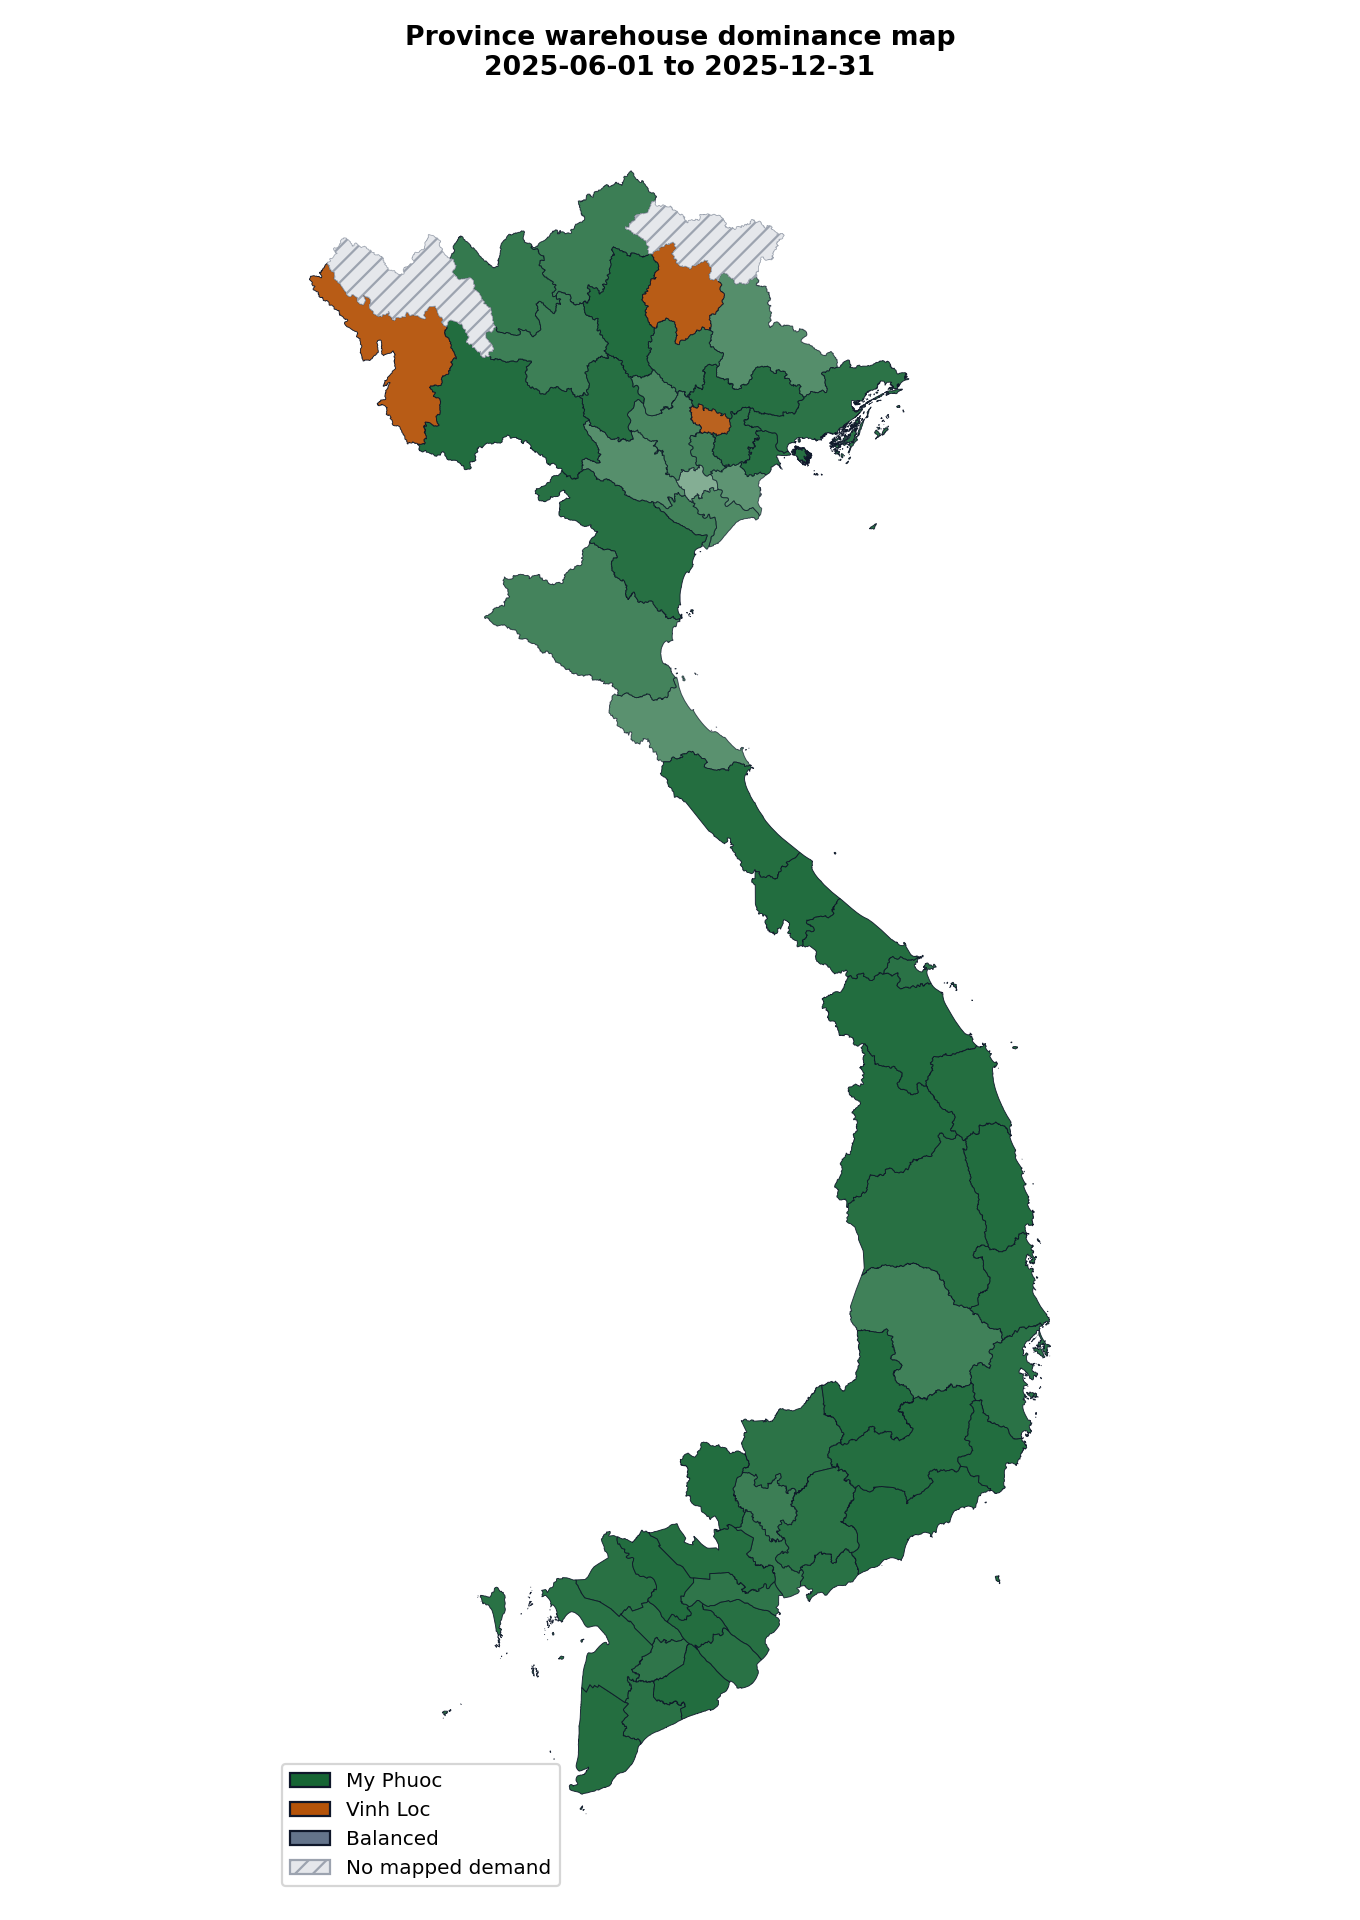
\includegraphics[width=0.5\linewidth,height=\textheight,keepaspectratio]{../charts/q12_warehouse_dominance_map.png}
\caption{Q1.2 Warehouse dominance map\label{fig:q12-wh-dominance}}
\end{figure}

\paragraph{Distance vs.~Demand Size
Correlation}\label{distance-vs.-demand-size-correlation}

We also analyze the relationship between delivery distance and order
characteristics. There is a clear spatial correlation between order size
(CBM) and delivery distance, showing that close-by urban centers (HCMC
and surrounding areas) order in higher density and frequency, as
illustrated in the scatter plot in Figure
\ref{fig:q12-dist-correlation}.

\begin{figure}
\centering
\pandocbounded{
\includegraphics[keepaspectratio]{../charts/q12_province_distance_correlation.png}}
\caption{Q1.2 Province distance
correlation\label{fig:q12-dist-correlation}}
\end{figure}

\paragraph{Urban vs.~Provincial Demand
Split}\label{urban-vs.-provincial-demand-split}

Finally, we segment the outbound volume into urban centers (HCMC, Hanoi,
Da Nang, Can Tho, Haiphong) versus the remaining provinces. As shown in
Figure \ref{fig:q12-urban-provincial}, urban centers drive a
disproportionately large and concentrated volume compared to the more
fragmented provincial demand.

\begin{figure}
\centering

\includegraphics[width=0.7\linewidth,height=\textheight,keepaspectratio]{../charts/q12_urban_provincial_split.png}
\caption{Q1.2 Urban and provincial
split\label{fig:q12-urban-provincial}}
\end{figure}

\begin{center}\rule{0.5\linewidth}{0.5pt}\end{center}

\subsection{Q1.3 Customer Segment Order Profile
Comparison}\label{q1.3-customer-segment-order-profile-comparison}

We compared the order profiles of \textbf{Modern Trade (MT)} (large
retail accounts like Co.op Mart, Lotte, etc.) and \textbf{Traditional
Trade / Distributor (TT)}.

\subsubsection{Key Profile Comparison
Table}\label{key-profile-comparison-table}

The comparison across the required dimensions is summarized below:

\begin{longtable}[]{@{}
  >{\raggedright\arraybackslash}p{(\linewidth - 4\tabcolsep) * \real{0.2857}}
  >{\centering\arraybackslash}p{(\linewidth - 4\tabcolsep) * \real{0.3571}}
  >{\centering\arraybackslash}p{(\linewidth - 4\tabcolsep) * \real{0.3571}}@{}}
\toprule\noalign{}
\begin{minipage}[b]{\linewidth}\raggedright
Dimension
\end{minipage} & \begin{minipage}[b]{\linewidth}\centering
Modern Trade (MT)
\end{minipage} & \begin{minipage}[b]{\linewidth}\centering
Traditional Trade / Distributor (TT)
\end{minipage} \\
\midrule\noalign{}
\endhead
\bottomrule\noalign{}
\endlastfoot
\textbf{Active Customers} & 117 & 253 \\
\textbf{Order Count} & 1315 & 3258 \\
\textbf{Avg. Order Quantity} & 65.02 units & 37.73 units \\
\textbf{Avg. Order Volume (CBM)} & 4.12 m³ & 1.91 m³ \\
\textbf{Avg. SKU Breadth / Order} & 3.09 SKUs & 4.43 SKUs \\
\textbf{Order Frequency (per customer/month)} & 1.87 & 2.15 \\
\textbf{Geographic Footprint} & 41 provinces / 6 regions & 57 provinces
/ 6 regions \\
\textbf{Avg. Delivery Distance} & 341.80 km & 298.76 km \\
\textbf{Pallet Share (\%)} & \textbf{69.17\%} & \textbf{40.44\%} \\
\textbf{Carton Share (\%)} & \textbf{27.57\%} & \textbf{51.49\%} \\
\textbf{Loose Share (\%)} & \textbf{3.25\%} & \textbf{8.07\%} \\
\end{longtable}

\subsubsection{Key Profile Insights}\label{key-profile-insights}

\begin{enumerate}
\def\labelenumi{\arabic{enumi}.}
\tightlist
\item
  \textbf{Order Size \& Consolidation}: Modern Trade orders are highly
  consolidated and large, averaging \textbf{65.02 units} and
  \textbf{4.12 CBM} per order. Traditional Trade orders are much smaller
  and fragmented, averaging \textbf{37.73 units} and \textbf{1.91 CBM}.
  This comparison of order metrics is visualised in Figure
  \ref{fig:q13-order-profile}.
\end{enumerate}

\begin{figure}
\centering

\includegraphics[width=0.85\linewidth,height=\textheight,keepaspectratio]{../charts/q13_order_profile_comparison.png}
\caption{Q1.3 Order profile comparison\label{fig:q13-order-profile}}
\end{figure}

\begin{enumerate}
\def\labelenumi{\arabic{enumi}.}
\setcounter{enumi}{1}
\item
  \textbf{Assortment Breadth vs.~Depth}: As shown in Figure
  \ref{fig:q13-order-profile}, Traditional Trade orders have a higher
  average SKU breadth (\textbf{4.43 SKUs} per order) than Modern Trade
  (\textbf{3.09 SKUs}). This indicates that TT customers order small
  quantities of a wide variety of SKUs, increasing warehouse sorting
  complexity.
\item
  \textbf{Packaging Unit Mix}: Modern Trade is highly pallet-centric,
  with \textbf{69.17\%} of their items shipped as full pallets.
  Traditional Trade is highly carton-centric (\textbf{51.49\%} of items)
  and has more loose picking (\textbf{8.07\%} vs.~3.25\% for MT). This
  breakdown of packaging unit selections is compared in Figure
  \ref{fig:q13-pkg-mix}.
\end{enumerate}

\begin{figure}
\centering
\pandocbounded{
\includegraphics[keepaspectratio]{../charts/q13_packaging_mix.png}}
\caption{Q1.3 Packaging mix\label{fig:q13-pkg-mix}}
\end{figure}

\begin{enumerate}
\def\labelenumi{\arabic{enumi}.}
\setcounter{enumi}{3}
\tightlist
\item
  \textbf{Geographic Spread}: Traditional Trade has a much wider
  geographic spread, covering \textbf{57 provinces} compared to MT's
  \textbf{41 provinces}, representing a highly fragmented, nation-wide
  distribution profile. The count of active provinces and regions for
  each segment is shown in Figure \ref{fig:q13-geo-spread}.
\end{enumerate}

\begin{figure}
\centering
\pandocbounded{
\includegraphics[keepaspectratio]{../charts/q13_geographic_spread.png}}
\caption{Q1.3 Geographic spread\label{fig:q13-geo-spread}}
\end{figure}

To see the spatial distribution of these sales, Figure
\ref{fig:q13-segment-geo-maps} shows the choropleth maps of MT and TT
customer demand across Vietnam.

\begin{figure}
\centering
\pandocbounded{
\includegraphics[keepaspectratio]{../charts/q13_segment_geographic_maps.png}}
\caption{Q1.3 Segment geography maps\label{fig:q13-segment-geo-maps}}
\end{figure}

\end{document}
